% 3-2-1 backup, and why RAID is not one.
% ---------------------------------------------------------------------------
% style.tex --- shared preamble for every figure in book/figures/tikz/
%
% One style for all figures: Latin Modern, thin black lines, a light grey
% fill, and one accent colour used only to mark what is untrusted or wrong.
% Build with scripts/build_figures.sh; see book/figures/README.md.
% ---------------------------------------------------------------------------
\documentclass[tikz,border=6pt]{standalone}
\usepackage[T1]{fontenc}
\usepackage{lmodern}
\usetikzlibrary{arrows.meta,positioning,shapes.geometric,calc,fit,backgrounds}

\hyphenpenalty=10000   % short lines in boxes: ragged, never hyphenated

\definecolor{lightgrey}{gray}{0.92}
\definecolor{accent}{HTML}{9B2D20}

\tikzset{
  every picture/.style={
    line width=0.6pt,
    font=\small,
    >={Stealth[length=5pt,width=4pt]},
    node distance=14pt and 24pt,
  },
  % shapes
  box/.style={draw, rectangle, inner xsep=8pt, inner ysep=5pt,
              minimum height=22pt, align=center},
  grey/.style={box, fill=lightgrey},
  rounded/.style={box, rounded corners=9pt},
  decision/.style={draw, diamond, aspect=2.4, inner sep=1.5pt, align=center},
  group/.style={draw, dashed, rounded corners=5pt, inner sep=7pt},
  % text
  tag/.style={font=\footnotesize, align=center, inner sep=2pt},
  note/.style={font=\footnotesize\itshape, align=center, inner sep=2pt},
  code/.style={font=\small\ttfamily},
  codetag/.style={font=\footnotesize\ttfamily, align=center, inner sep=2pt},
  title/.style={font=\small\scshape, align=center, inner sep=2pt},
  % lines
  arrow/.style={->},
  back/.style={->, dashed},
  thin/.style={line width=0.4pt, gray},
  % the one accent, for what is untrusted, wrong or missing
  bad/.style={accent},
  badbox/.style={box, draw=accent, text=accent},
}

\begin{document}
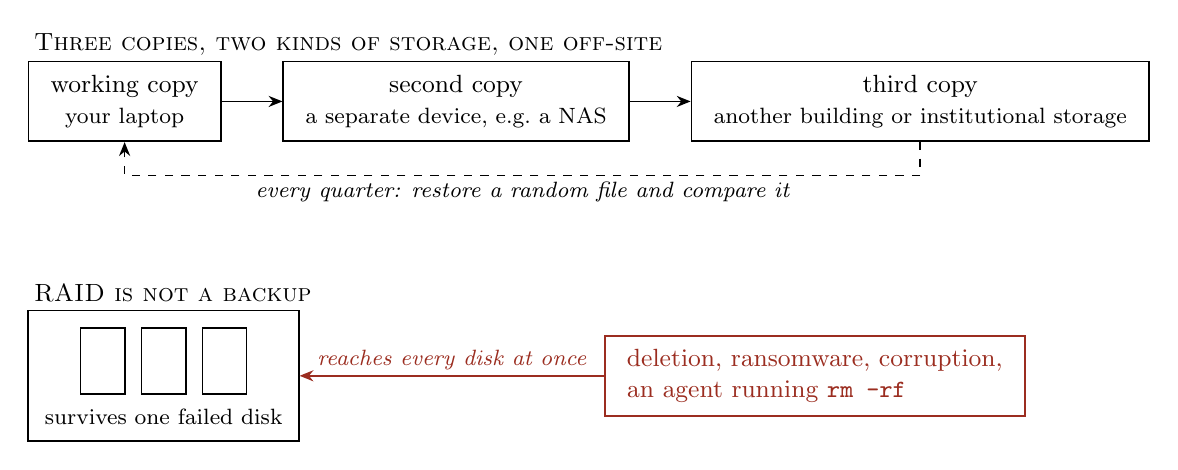
\begin{tikzpicture}[node distance=10pt and 22pt]
  \node[title, anchor=west] (t1) at (0,0) {Three copies, two kinds of storage, one off-site};
  \node[box, below=6pt of t1.west, anchor=north west] (w) {working copy\\ \footnotesize your laptop};
  \node[box, right=of w] (n) {second copy\\ \footnotesize a separate device, e.g.\ a NAS};
  \node[box, right=of n] (o) {third copy\\ \footnotesize another building or institutional storage};
  \draw[->] (w) -- (n);
  \draw[->] (n) -- (o);
  \draw[back] (o.south) -- ++(0,-12pt) -| node[note, pos=0.25, below] {every quarter: restore a random file and compare it} (w.south);

  \node[title, anchor=west] (t2) at (0,-90pt) {RAID is not a backup};
  \node[box, below=6pt of t2.west, anchor=north west, inner sep=6pt] (raid) {%
    \tikz[baseline]{\foreach \i in {0,1,2} \draw (\i*22pt,0) rectangle ++(16pt,24pt);}\\
    \footnotesize survives one failed disk};
  \node[badbox, right=110pt of raid, align=left] (bad) {deletion, ransomware, corruption,\\an agent running \texttt{rm -rf}};
  \draw[->, bad] (bad) -- node[note, above, text=accent] {reaches every disk at once} (raid);
\end{tikzpicture}
\end{document}
